% 五号字体,开明式标点处理,不设置默认字体
\documentclass[UTF8,12pt,punct=kaiming,fontset=none]{ctexart}
\usepackage{fontspec}  % 字体
\usepackage{subcaption}  % 节标题
% 品红色链接和注释
% \usepackage[colorlinks=true, linkcolor=magenta, citecolor=magenta, urlcolor=magenta]{hyperref}
% 黑色链接和注释
\usepackage[colorlinks=true, linkcolor=black, citecolor=black, urlcolor=black]{hyperref}
\usepackage{geometry}  % 页面布局
\usepackage{fancyhdr}  % 页眉页脚
\usepackage{titlesec}  % 标题
\usepackage{caption}  % 图表标题
\usepackage{floatrow}  % 图表排版
\usepackage{graphicx}  % 图片路径
% 表格(可选)
\usepackage{multirow}
\usepackage{boldline}
% 电路图(可选)
\usepackage{tikz}
\usepackage[european,nooldvoltagedirection]{circuitikz}

% 图片路径
\graphicspath{{figures/}}

% 字体
\setCJKmainfont{Source Han Serif SC}
\setCJKsansfont{Source Han Sans SC}
\setmainfont{CMU Serif}

% 布局
\geometry{a4paper,left=2cm,right=2cm,top=2.5cm,bottom=2.5cm}
\setlength{\headheight}{25pt}

% 图表标题
\DeclareCaptionFont{captionfont}{\small}
\captionsetup{font=captionfont}
\floatsetup{style=plaintop}

% 页眉页脚
\pagenumbering{arabic}
\pagestyle{fancy}
\fancyhead[L]{· \hspace{0.1cm} \thepage \hspace{0.1cm} ·}
\fancyhead[C]{红石数电评论\\\scriptsize{Review of Redstonic Digital Circuit}}
\fancyhead[R]{第1期\\\scriptsize{2022年1月}}
\fancyfoot[L,C,R]{}

% 首页页码
\setcounter{page}{1}

% 标题
\title{\vspace{-1.5cm}基于RV32M标准的运算器实现\vspace{-0.5cm}}
\author{@MorQin\footnote{作者联系方式\url{https://space.bilibili.com/14122148}},@Nikkeru\footnote{先进红石数电技术研讨组ARS}}
\date{}

% 参考文献标注
\newcommand*{\upcite}[1]{
    \textsuperscript{\cite{#1}}
}

\begin{document}
\maketitle
\thispagestyle{fancy} % 首页页眉页脚
\vspace{-0.7cm}

% 摘要及关键词
\begin{flushright}
    \begin{minipage}[c]{0.91\linewidth}
        \titleformat{\section}[leftmargin]{\sffamily\small\bfseries}{}{0cm}{}
        \titlespacing{\section}{1.5cm}{1ex}{0cm}

        \section{摘 \hspace{0.105cm} 要}
        \small 本文将简要\footnotemark[1]介绍两种算法分别用于实现乘法器与除法器。

        \section{关键词}
        \small 关键词 \hspace{0.5cm} 关键词
    \end{minipage}
\end{flushright}
\vspace{0.2cm}

% 节标题格式
\titleformat{\section}[hang]{\large\sffamily\bfseries}{\textmd{\thesection}}{0.5cm}{}
\titlespacing{\section}{0cm}{0.5ex}{0.2ex}
\titleformat{\subsection}[hang]{\normalsize\sffamily}{\textmd{\thesubsection}}{0.5cm}{}
\titlespacing{\subsection}{0cm}{0.5ex}{0.2ex}
\setcounter{section}{0}

\footnotetext[1]{欲知更多细节请联系作者}

\section{引言}
RISC-V是一个基于精简指令集(RISC)原则的开源指令集架构(ISA)\upcite{patterson2017risc}。
RV32M是RISC-V指令集中的一个标准扩展,它包含了整数乘法和除法两类算术,一共八条指令,见图\ref{fig1}。
对于乘法而言,操作数可能是有符号乘无符号,而并非同数集。对于除法而言就比较简单了,操作数所使用的数集一致。两者的共同点在于运算后产生的结果分为两部分:对于乘法是高低位积,对于除法是商和余数,选取哪一部分则由不同的指令决定。在Minecraft(MC)中实现\upcite{RLC}乘除法是比较容易的,使用简单的移位累加和试减法即可,但这些基础的算法并不能简便的实现补码运算,所以本文引入比较常见的Booth和Nonrestoring(不恢复余数)算法。

\begin{figure}[H]
    \centering
    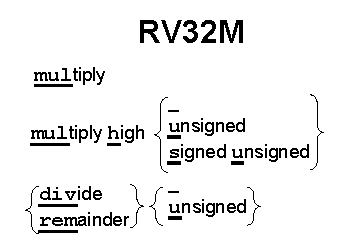
\includegraphics[scale=1]{RV32M.pdf}
    \caption{RV32M 指令的图示}
    \label{fig1}
\end{figure}

\section{算法与架构设计}
为方便实现有/无符号的运算,我们将操作数统一扩展成33bit补码数。无论操作数原本有无符号,它们都能用33bit的补码数表示,唯一要多加的逻辑仅是根据指令需求来控制操作数的符号位扩展与否。文章实现的算法仅对MC有效,切勿直接代入现实电路。
\newline

\textbf{乘法:}

在基础的移位累加算法中,有纯并行和纯串行两种实现方案,我们以纯串行为基础,如图\ref{fig2}.(a)。为了实现Booth算法,我们仅需改造累加器的输入控制即可,如图\ref{fig2}.(b)。上诉方案可算作 Radix2 Booth的一种实现,为了加速乘法,算法\cite{parhami2010computer}界有很多技术,本文所使用并实现的是Radix4 Booth部分树串行方案。
\newline
\begin{figure}[H]
    \centering
    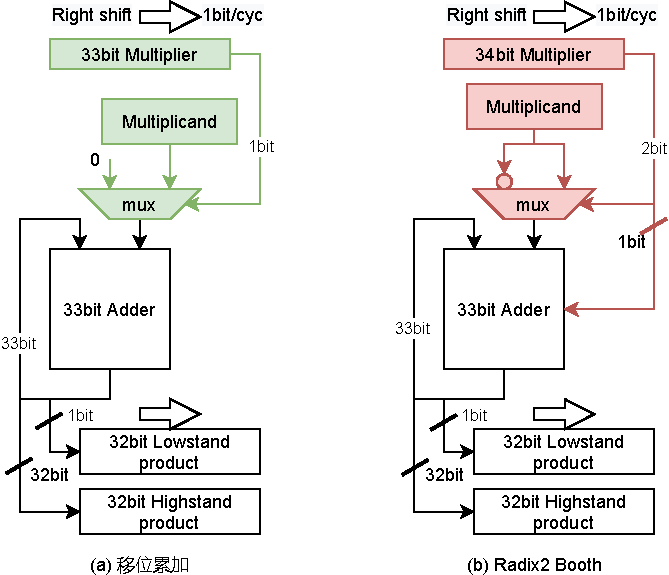
\includegraphics[scale=1]{mul.pdf}
    \caption{乘法器算法对比}
    \label{fig2}
\end{figure}

乘法方案使用的是普通树,并非CSA(进位保留加法器)树。部分树是对全树的剪支复用,那么部分树的深度也就决定了成品模块的总延迟以及频率。乘法方案使用的是深度为4的部分树(基础方案的深度可视作1)。树之后的部分与基础串行方案类似,不同之处仅在于每次\footnote{模块内为精确时序,内部有多个时钟,此处为8t(时钟周期)}的位移量。
整体预览如图\ref{fig3}。
\begin{figure}[H]
    \centering
    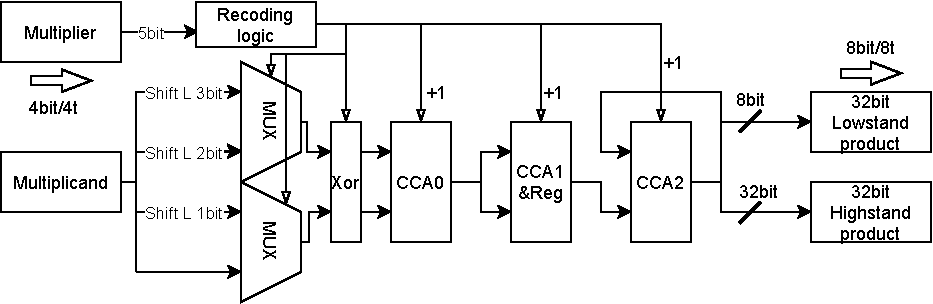
\includegraphics[scale=1]{hmul.pdf}
    \caption{Radix4 Booth部分树串行乘法}
    \label{fig3}
\end{figure}
\newpage

\textbf{除法:}

类似乘法,我们以串行试减法(恢复余数法)为基础,如图\ref{fig4}.(a)。为实现不恢复余数算法,我们不仅需要改造累加器的输入控制,还需要加入一些控制逻辑(图内未画完整)如图\ref{fig4}.(b)。想要加速除法并不容易,因为它不像乘法那样可以拆解并行化,但也并非无法,算法界的加速技术很多,本文所使用并实现的是部分余数选择不恢复余数方案\footnote{此名称非正式,仅参考自进位选择加法器}。
\begin{figure}[H]
    \centering
    \begin{subfigure}{3in}
        \centering
        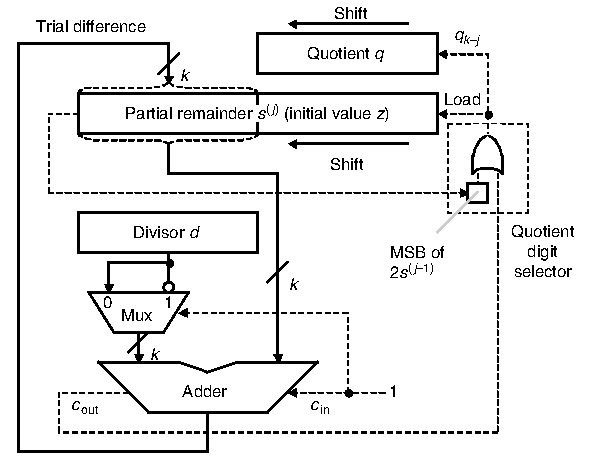
\includegraphics[width=\linewidth]{div1.pdf}
        \caption{恢复余数法}
        \label{fig:a}
    \end{subfigure}
    %\hspace{1cm}
    \begin{subfigure}{2.5in}
        \centering
        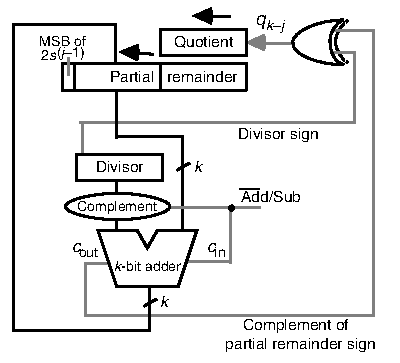
\includegraphics[width=\linewidth]{div2.pdf}
        \caption{不恢复余数法}
        \label{ubfig:b}
    \end{subfigure}
    \caption{除法器算法对比\cite{parhami2010computer}}
    \label{fig4}
\end{figure}

不恢复余数算法每周期的逻辑电路可以简化成图\ref{fig5}.(a)的样式。本周期的选择信号来自上一周期逻辑黑盒的输出结果。一般不恢复余数算法中的控制流类似图\ref{fig5}.(b)\footnote{计算:等待计算完成。传递:选择信号的传输延迟}中的上半部分(原始)。若想缩短控制流每周期的延迟,就得想办法优化掉计算这一步。图\ref{fig5}.(a)中的逻辑黑盒内有两步操作:计算、选择,无论先进行哪一步都可以,只要保证最后输出一致。因此可以将控制流改进为类似图\ref{fig5}.(b)中的下半部分(改进后)。

\begin{figure}[H]
    \centering
    \begin{subfigure}{6cm}
        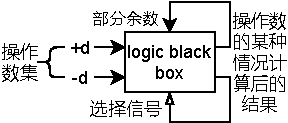
\includegraphics[width=\linewidth]{divb.pdf}
        \caption{不恢复余数除法器简化电路}
        \label{fig5:a} %% label for first subfigure
    \end{subfigure}
    \hspace{0.5in}%使第一个子图占一半空间
    \begin{subfigure}{8cm}
        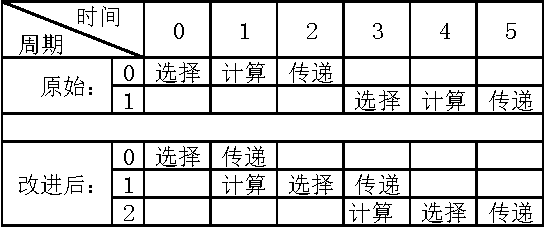
\includegraphics[width=\linewidth]{divt.pdf}
        \caption{时序对比}
        \label{fig5:subfig:b} %% label for secondsubfigure
    \end{subfigure}
    \caption{}
    \label{fig5} %% label for entire figure
\end{figure}

%不恢复余数算法中每周期除数的输入选择,由上次计算结果中的符号位决定。上周期的结果出来后,需要经过一段控制信号传递以及除数选择器的延迟,这一周期的除数才真正输入到累加器中。中间那段延迟非常大,直接消除延迟是不太可能的,但可以在每周期内隐藏这段延迟。因为除数的输入只有两种情况(+d,-d),所以将两种情况都计算一次,除数选择器消失了,但现在每周期运算后有两个结果(部分余数)。自然的,上周期结果控制的对象从除数变成了部分余数。直观的来说就是在每周期中,提前计算每一种情况,并将选择这一步骤滞后,滞后到选择器结果一出就立马进行下一周期的计算。通过图\ref{fig5}(时序)可看出,对于单次运算的延迟有可观的改善。
实现先计算后选择的办法便是将+d和-d这两种情况都计算一次,对计算后的结果进行选择。因此实现部分余数选择不恢复余数算法仅需要多加一个累加器与少量控制逻辑即可,其它部分与基础算法类似。整体预览如图\ref{fig6}。
\begin{figure}[h]
    \centering
    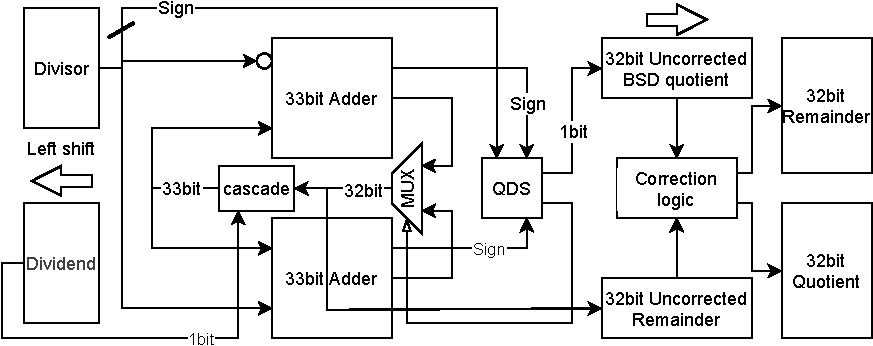
\includegraphics[scale=1]{div.pdf}
    \caption{部分余数选择不恢复余数除法}
    \label{fig6}
\end{figure}

\begin{figure}[H]
    \centering
    \begin{subfigure}{3in}
        \label{fig7:a} %% label for first subfigure
        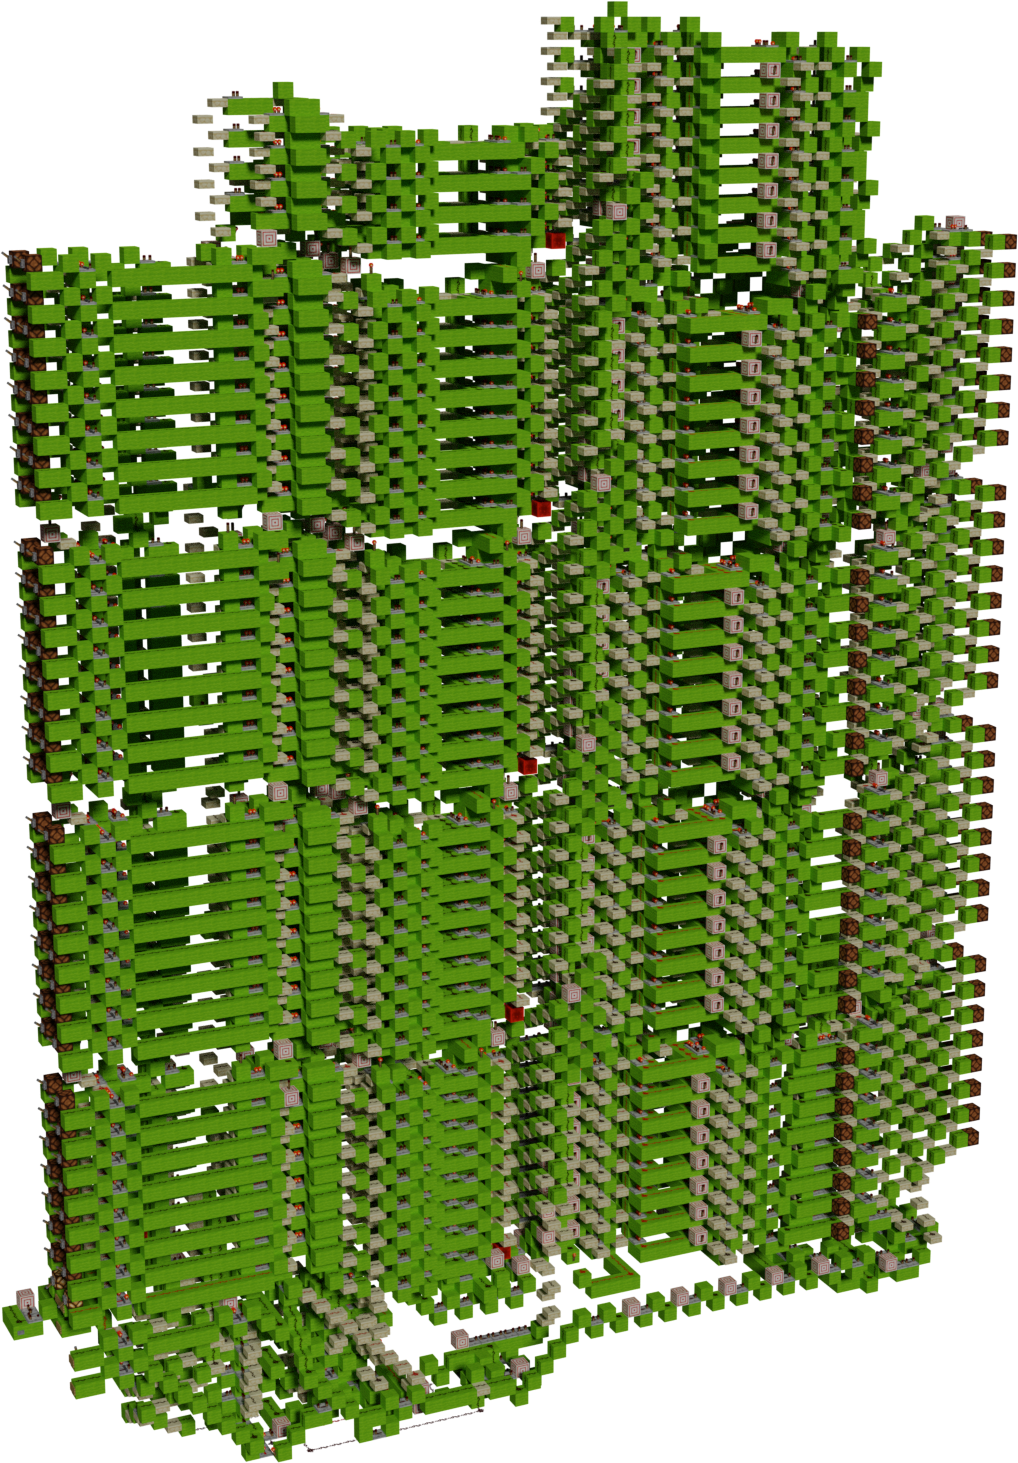
\includegraphics[width=\linewidth]{R4PTS.png}
        \caption{乘法器}
    \end{subfigure}
    \hspace{1in}%使第一个子图占一半空间
    \begin{subfigure}{1.5in}
        \label{fig7:subfig:b} %% label for secondsubfigure
        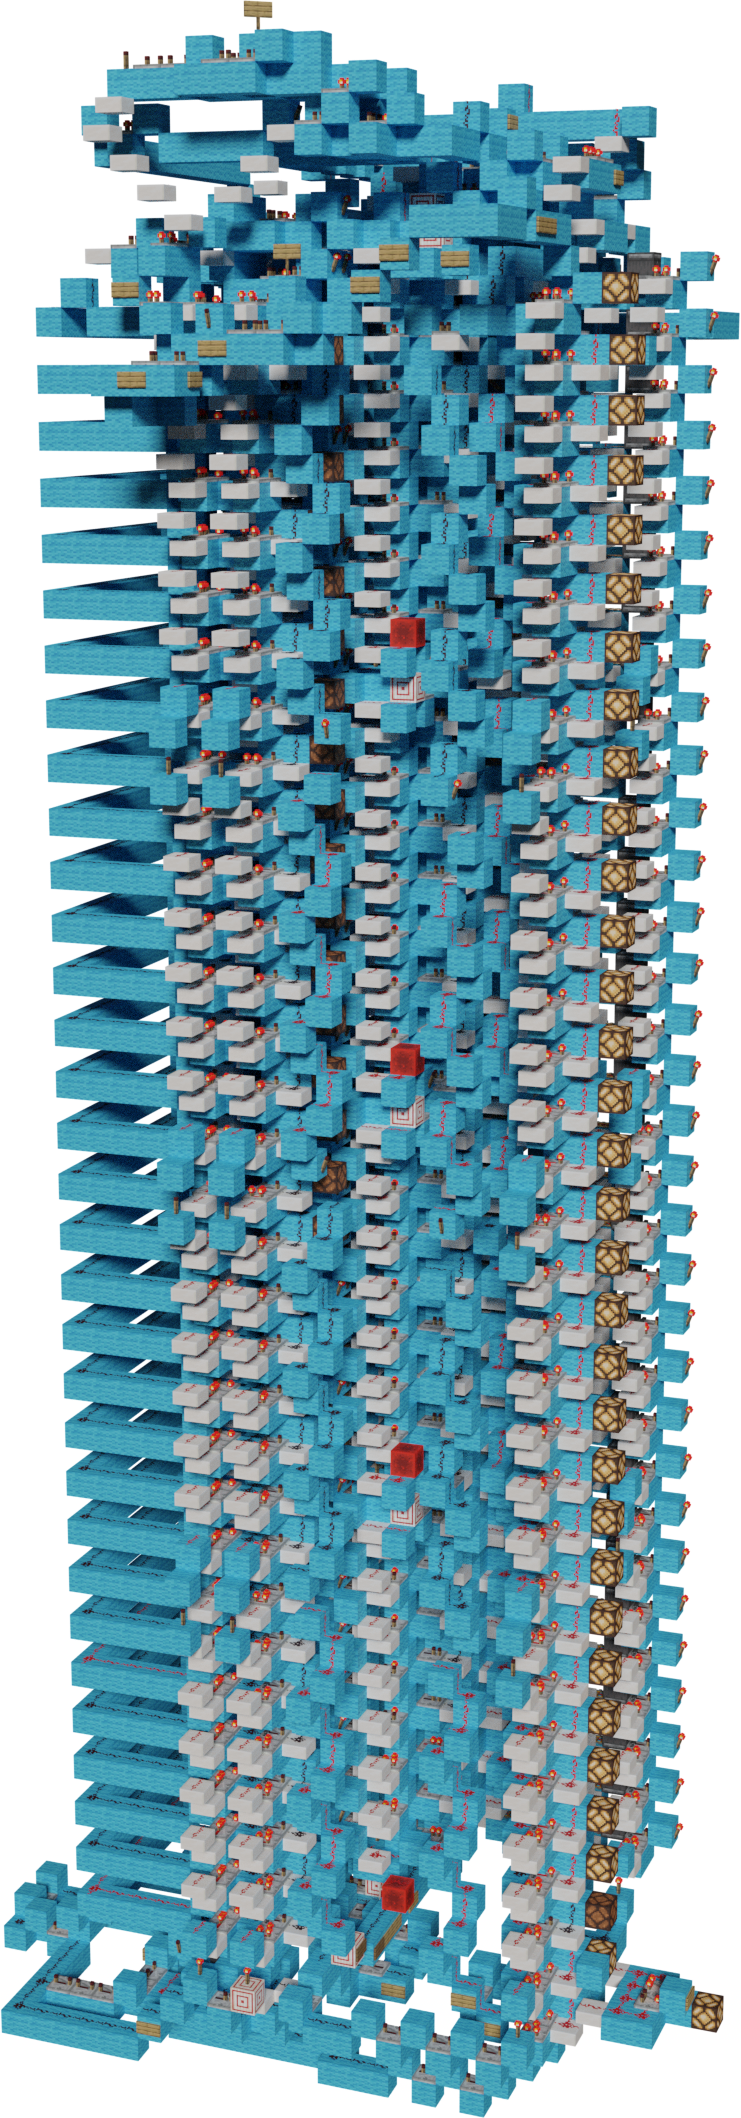
\includegraphics[width=\linewidth]{PSN.png}
        \caption{除法器(无修正模块)}
    \end{subfigure}
    \caption{成品模块展示}
    \label{fig7} %% label for entire figure
\end{figure}

\section{实例概览}

乘法器成品模块\footnote{获取模块请联系作者}如图\ref{fig7}.(a)。整体宽度保持在9个方块,长和高分别是130,98。性能:总延迟100t,流水间隔40t。模块因观感和体积原因使用了可能不太稳定的2t(间隔变化)移位寄存器。实际使用中,玩家可自行更改为其它稳定移位模块(数据在图\ref{fig3}中)。

除法器半成品模块如图\ref{fig7}.(b)。图示模块为除法器核心,相对于完成品仅缺少结果修正模块。长宽可动态设计,高度约80Block。
单次运算延迟9t,预计完成品总延迟350t以内,单周期模块。
除法器的实现参考自Nikkeru(原型建于SBT\footnote{Sitetechnology brickmoving team}服务器中)。

\section{总结}
本文所实现的乘法器速度不比串行CSA乘法器\footnote{相关介绍\url{https://www.bilibili.com/video/BV1nv411t7pk}}快很多。在付出多倍体积的代价下,机器极大地提高了流水性能。
除法器在仅多用了一个CCA的情况下实现了更优的总延迟。
这类高性能运算器能为红石计算器、CPU提供更为强大的性能。
\newline

致谢:感谢主编辰占鳌头的多次审稿,提出的诸多建议使得文章可读性提升了数倍。感谢Resens和Nikkeru的技术帮助。

\bibliographystyle{unsrt}
\bibliography{reference.bib}
\end{document}